\documentclass[aspectratio=169, lualatex, handout]{beamer}
\makeatletter\def\input@path{{theme/}}\makeatother\usetheme{cipher}

\title{Applied Cryptography}
\author{Nadim Kobeissi}
\institute{American University of Beirut}
\instituteimage{images/aub_white.png}
\date{\today}
\coversubtitle{CMPS 297AD/396AI\\Fall 2025}
\coverpartname{Part 2: Real-World Cryptography}
\covertopicname{2.7: Cryptocurrency Cryptography}
\coverwebsite{https://appliedcryptography.page}

\begin{document}
\begin{frame}[plain]
	\titlepage
\end{frame}

\section{Bitcoin}

\begin{frame}{The problem: trust in digital commerce}
	\begin{itemize}
		\item Online commerce relies entirely on financial institutions as trusted third parties.
		\item Banks, payment processors, credit card companies mediate every transaction.
		\item This trust-based model has fundamental limitations:
		      \begin{itemize}
			      \item Intrinsic dependence on centralized parties.
			      \item Financial institutions must mediate disputes.
			      \item Increases transaction costs significantly.
		      \end{itemize}
	\end{itemize}
\end{frame}

\begin{frame}{Weaknesses of the trust-based model}
	\begin{itemize}
		\item \textbf{High transaction costs}: Mediation costs make micropayments impractical.
		\item \textbf{Reversibility spreads distrust}: Merchants need extensive customer information.
		\item \textbf{Fraud is inevitable}: Some percentage of fraud accepted as cost of business.
		\item \textbf{No digital cash equivalent}: Physical cash works person-to-person, but no digital. analog exists
	\end{itemize}
\end{frame}

\begin{frame}{Peer-to-peer electronic cash}
	\begin{itemize}
		\item Replace trust with cryptographic proof.
		\item Enable direct transactions between parties without intermediaries.
		\item Key properties needed:
		      \begin{itemize}
			      \item Computationally impractical to reverse (protects sellers).
			      \item Optional escrow mechanisms (protects buyers).
			      \item No reliance on third parties.
		      \end{itemize}
	\end{itemize}
\end{frame}

\begin{frame}{Core challenge: double spending}
	\begin{itemize}
		\item Digital information can be copied perfectly.
		\item Without a central authority, how do we prevent spending the same coin twice?
		\item Traditional solution: Central mint/bank tracks all transactions.
		\item Problem: This reintroduces the trusted third party.
	\end{itemize}
\end{frame}

\begin{frame}{Bitcoin's solution}
	\begin{itemize}
		\item Peer-to-peer distributed timestamp server.
		\item Generates computational proof of transaction order.
		\item Security assumption: Honest nodes control majority of CPU power.
		\item Key innovations:
		      \begin{itemize}
			      \item Proof-of-work consensus mechanism.
			      \item Blockchain as public ledger.
			      \item Economic incentives for honest behavior.
		      \end{itemize}
	\end{itemize}
\end{frame}

\begin{frame}{Historical context}
	\begin{itemize}
		\item Published October 31, 2008 by Satoshi Nakamoto (pseudonym)
		\item Built on decades of cryptographic research:
		      \begin{itemize}
			      \item Digital signatures (ECDSA)
			      \item Hashcash proof-of-work (Adam Back, 1997)
			      \item Cryptographic timestamps (Haber \& Stornetta, 1991)
			      \item B-money and bit gold proposals (Wei Dai, Nick Szabo)
		      \end{itemize}
		\item First practical solution to Byzantine Generals Problem for money.
	\end{itemize}
\end{frame}

\begin{frame}{The Byzantine Generals Problem}
	\begin{itemize}
		\item Classical problem in distributed computing (Lamport, Shostak, Pease, 1982).
		\item Scenario: Byzantine generals must coordinate attack on a city.
		      \begin{itemize}
			      \item Generals can only communicate via messengers.
			      \item Some generals may be traitors sending false messages.
			      \item Need consensus: all loyal generals execute same plan.
		      \end{itemize}
		\item Core challenge: How to achieve reliable consensus when:
		      \begin{itemize}
			      \item Communication channels are unreliable.
			      \item Some participants may be malicious.
			      \item No central authority to trust.
		      \end{itemize}
		\item \textbf{Bitcoin's breakthrough}: First practical solution for digital money using proof-of-work.
	\end{itemize}
\end{frame}

\subsection{Proof-of-Work}

\begin{frame}{What is proof-of-work?}
	\begin{itemize}
		\item A computational puzzle that takes significant effort to solve.
		\item Core component of blockchain consensus (for PoW-based chains).
		\item Properties:
		      \begin{itemize}
			      \item Hard to compute (requires many attempts).
			      \item Easy to verify (single check).
			      \item Difficulty adjustable.
		      \end{itemize}
		\item Creates a cost for participation \rightarrow\ prevents spam/attacks.
	\end{itemize}
\end{frame}

\begin{frame}{How proof-of-work functions}
	\begin{itemize}
		\item PoW is a hash function with:
		      \begin{itemize}
			      \item \textbf{Fixed inputs}: Block header data (transactions, timestamp, etc.)
			      \item \textbf{Variable input}: Nonce (number used once)
			      \item \textbf{Constraint}: Output must match specific pattern (e.g. start with a specific number of zeroes)
		      \end{itemize}
		\item Process:
		      \begin{enumerate}
			      \item Hash(fixed inputs + nonce)
			      \item Check if output meets constraint
			      \item If not, increment nonce and repeat
			      \item If yes, you've found the proof!
		      \end{enumerate}
	\end{itemize}
\end{frame}

\begin{frame}{Bitcoin's proof-of-work constraint}
	\begin{itemize}
		\item Bitcoin uses double SHA-256: \func{sha256}{\func{sha256}{\texttt{data}}}
		\item Constraint: Hash value < target threshold
		\item Can be visualized as ``leading zeros'':
		      \begin{itemize}
			      \item Hash as 256-bit number in big-endian
			      \item More leading zeros = smaller number
			      \item More leading zeros = harder to find
		      \end{itemize}
		\item Example outputs:
		      \begin{itemize}
			      \item \texttt{00000000000000000007b...} (valid - many zeros)
			      \item \texttt{5fec4ba9f3c2d8a1b9e7...} (invalid - no leading zeros)
		      \end{itemize}
	\end{itemize}
\end{frame}

\begin{frame}{Real Bitcoin difficulty numbers}
	\begin{itemize}
		\item Example from 2022:
		      \begin{itemize}
			      \item Difficulty: 34,244,331,613,176 (\approx$2^{45}$)
			      \item Actual target: difficulty \times\ $2^{32}$ = $2^{77}$
			      \item Hash must be less than $2^{77}$ (out of $2^{256}$ possible)
		      \end{itemize}
		\item This means:
		      \begin{itemize}
			      \item Network computes \approx$2^{77}$ hashes per block
			      \item That's 150,000,000,000,000,000,000,000 hashes!
			      \item All to find one valid nonce
		      \end{itemize}
	\end{itemize}
\end{frame}

\begin{frame}{The mining algorithm}
	\begin{itemize}
		\item Input components:
		      \begin{itemize}
			      \item Version number
			      \item Previous block hash
			      \item Merkle root of transactions
			      \item Timestamp
			      \item Difficulty target
			      \item \textbf{Nonce} (32-bit number)
		      \end{itemize}
		\item Mining loop:
		      \begin{enumerate}
			      \item Set nonce = 0
			      \item Compute hash = \func{sha256}{\func{sha256}{\texttt{header}}}
			      \item If hash < target, success!
			      \item Else, \texttt{nonce++}, go to step 2
		      \end{enumerate}
	\end{itemize}
\end{frame}

\begin{frame}{Why is proof-of-work necessary?}
	\begin{itemize}
		\item Without PoW, blocks could be created instantly:
		      \begin{itemize}
			      \item Anyone could rewrite history at will
			      \item No way to determine ``canonical'' chain
			      \item Double-spending would be trivial
		      \end{itemize}
		\item PoW provides:
		      \begin{itemize}
			      \item \textbf{Finality}: Expensive to reverse transactions
			      \item \textbf{Sybil resistance}: Can't fake computational work
			      \item \textbf{Fair lottery}: Proportional to hashpower
			      \item \textbf{Time spacing}: Predictable block intervals
		      \end{itemize}
	\end{itemize}
\end{frame}

\begin{frame}{The double-spending problem revisited}
	\begin{itemize}
		\item Without PoW:
		      \begin{enumerate}
			      \item Alice sends 1 BTC to Bob (Transaction A)
			      \item Alice creates alternate history sending same 1 BTC to herself (Transaction B)
			      \item Both histories equally valid \rightarrow\ no consensus
		      \end{enumerate}
		\item With PoW:
		      \begin{enumerate}
			      \item Transaction A gets included in block N
			      \item To double-spend, Alice must:
			            \begin{itemize}
				            \item Re-mine block N with Transaction B
				            \item Re-mine all subsequent blocks
				            \item Do this faster than honest network
			            \end{itemize}
			      \item Cost grows exponentially with confirmations
		      \end{enumerate}
	\end{itemize}
\end{frame}

\begin{frame}{Proof-of-work as a random lottery}
	\begin{itemize}
		\item Each hash attempt is like a lottery ticket:
		      \begin{itemize}
			      \item Probability of success = target / $2^{256}$
			      \item Independent trials (memoryless)
			      \item No progress - each attempt equally likely
		      \end{itemize}
		\item Properties:
		      \begin{itemize}
			      \item Can't predict who will win
			      \item Can't get ``closer'' to solution
			      \item More hashpower = more tickets/second
			      \item Fair: winning probability $\propto$ hashpower
		      \end{itemize}
	\end{itemize}
\end{frame}

\begin{frame}{The economics of mining}
	\begin{itemize}
		\item Mining costs:
		      \begin{itemize}
			      \item Hardware (ASICs, GPUs)
			      \item Electricity (biggest ongoing cost)
			      \item Cooling and infrastructure
			      \item Opportunity cost of capital
		      \end{itemize}
		\item Mining rewards:
		      \begin{itemize}
			      \item Block subsidy (currently 3.125 BTC)
			      \item Transaction fees
		      \end{itemize}
		\item Equilibrium: Total mining cost ≈ Total mining revenue
		\item This ensures appropriate security level
	\end{itemize}
\end{frame}

\begin{frame}{Bitcoin mining at peak consumption}
	\begin{columns}[c]
		\begin{column}{1\textwidth}
			\begin{itemize}
				\item \textbf{Peak consumption scenarios}:
				      \begin{itemize}
					      \item During 2021 bull run: \approx180 TWh/year\footnote{\url{https://www.statista.com/statistics/881472/worldwide-bitcoin-energy-consumption/}}
					      \item More than entire power consumption of Argentina (121 TWh)
					      \item Exceeds Netherlands (117 TWh) + UAE (120 TWh) combined
				      \end{itemize}
				\item \textbf{Single mining facilities}:
				      \begin{itemize}
					      \item Riot Platforms Texas facility: 700 MW capacity
					      \item Equivalent to powering 500,000 US homes
					      \item Marathon Digital: 500+ MW across facilities
				      \end{itemize}
				\item \textbf{Regional impacts}:
				      \begin{itemize}
					      \item Kazakhstan (2021): 18\% of global hashrate\footnote{\url{https://thediplomat.com/2021/11/kazakhstans-power-shortages-crypto-miners-and-geopolitics/}}
					      \item Caused nationwide power shortages
					      \item Government imposed mining restrictions
				      \end{itemize}
			\end{itemize}
		\end{column}
	\end{columns}
\end{frame}

\begin{frame}{ASIC resistance: Alternative PoW designs}
	\begin{itemize}
		\item Problem: Bitcoin mining dominated by specialized hardware (ASICs)
		\item Goal: Make mining accessible to regular computers
		\item Approaches:
		      \begin{itemize}
			      \item \textbf{Memory-hardness}: Require large amounts of RAM
			      \item \textbf{Algorithm complexity}: Use operations ASICs struggle with
			      \item \textbf{Regular changes}: Modify algorithm periodically
		      \end{itemize}
		\item Trade-offs:
		      \begin{itemize}
			      \item More democratic vs. less efficient
			      \item Decentralization vs. security
		      \end{itemize}
	\end{itemize}
\end{frame}

\begin{frame}{Memory-hard proof-of-work}
	\begin{columns}[c]
		\begin{column}{1\textwidth}
			\begin{itemize}
				\item Example: Ethereum's Ethash (before ``proof-of-stake''\footnote{We will discuss what ``proof-of-stake'' is later in this slideshow.} transition)
				\item How it works:
				      \begin{enumerate}
					      \item Generate large dataset (\approx4GB)
					      \item Mining requires random access to dataset
					      \item Can't compute on-the-fly (too slow)
					      \item Must store entire dataset in memory
				      \end{enumerate}
				\item Why it resists ASICs:
				      \begin{itemize}
					      \item Memory is expensive (can't optimize much)
					      \item Memory bandwidth becomes bottleneck
					      \item Levels playing field between ASICs and GPUs
				      \end{itemize}
			\end{itemize}
		\end{column}
	\end{columns}
\end{frame}

\begin{frame}{Virtual machine based PoW}
	\begin{itemize}
		\item Example: RandomX (used by Monero)
		\item Concept:
		      \begin{itemize}
			      \item Create custom instruction set
			      \item PoW executes random program
			      \item Optimized for CPU architecture
		      \end{itemize}
		\item Implementation:
		      \begin{enumerate}
			      \item Generate random program from block data
			      \item Execute program many times
			      \item Result must meet difficulty target
		      \end{enumerate}
		\item Advantage: CPUs excel at general computation
		\item Disadvantage: More complex, harder to verify
	\end{itemize}
\end{frame}

\begin{frame}{From proof-of-work to consensus}
	\begin{itemize}
		\item PoW doesn't directly create consensus
		\item Instead, it enables consensus through:
		      \begin{enumerate}
			      \item Making blocks expensive to create
			      \item Creating unforgeable chain of work
			      \item Allowing objective comparison of chains
			      \item Economically punishing dishonest behavior
		      \end{enumerate}
		\item The ``longest chain rule'' works because:
		      \begin{itemize}
			      \item Longest = most cumulative work
			      \item Most work = most resources spent
			      \item Rational miners extend longest chain
		      \end{itemize}
	\end{itemize}
\end{frame}

\subsection{Coins as Digital Signature Chains}

\begin{frame}{Electronic coins as digital signatures}
	\begin{itemize}
		\item Bitcoin defines an electronic coin as a chain of digital signatures.
		\item Each owner transfers the coin by:
		      \begin{itemize}
			      \item Digitally signing a hash of the previous transaction.
			      \item Adding the next owner's public key.
			      \item Appending this to the end of the coin.
		      \end{itemize}
		\item The payee can verify ownership by checking the chain of signatures.
	\end{itemize}
\end{frame}

\begin{frame}{Transaction structure}
	\begin{itemize}
		\item \textbf{Transaction inputs}: References to previous transactions.
		\item \textbf{Transaction outputs}: Amount and recipient's public key hash.
		\item \textbf{Digital signature}: Proves the owner authorized the transfer.
		\item Coins don't exist as discrete units, only as transaction chains.
	\end{itemize}
\end{frame}

\begin{frame}{A coin is the set of its transactions}
	\bigimagewithcaption{bitcoin_transactions.png}{Source: Satoshi Nakamoto}
\end{frame}

\begin{frame}{How are coins created?}
	\begin{columns}[c]
		\begin{column}{1\textwidth}
			\begin{itemize}
				\item New coins are created through \textbf{mining} - the process of adding blocks to the blockchain.
				\item Each block contains a special \textbf{coinbase transaction}\footnote{Not to be confused with Coinbase, the American cryptocurrency exchange company of the same name.}:
				      \begin{itemize}
					      \item First transaction in every block.
					      \item Has no inputs (creates coins from nothing).
					      \item Rewards the miner with newly minted bitcoins.
				      \end{itemize}
			\end{itemize}
		\end{column}
	\end{columns}
\end{frame}

\begin{frame}{The coinbase transaction in detail}
	\begin{itemize}
		\item \textbf{Structure of coinbase transaction}:
		      \begin{itemize}
			      \item No inputs (creates coins ex nihilo).
			      \item Single output to miner's address.
			      \item Can include arbitrary data in coinbase field.
			      \item Must be first transaction in block.
		      \end{itemize}
		\item \textbf{Mining process}:
		      \begin{enumerate}
			      \item Miner collects pending transactions from mempool.
			      \item Creates coinbase transaction paying themselves.
			      \item Builds block with coinbase tx + other transactions.
			      \item Searches for valid proof-of-work nonce. \leftarrow\ (this is what ``mining'' is about)
			      \item Broadcasts valid block to network.
		      \end{enumerate}
	\end{itemize}
\end{frame}

\begin{frame}{From nonce to Bitcoin: the complete process}
	\begin{itemize}
		\item \textbf{Step 1: Block construction}
		      \begin{itemize}
			      \item Miner creates coinbase transaction paying themselves.
			      \item Adds other pending transactions from mempool.
			      \item Builds Merkle tree of all transactions.
			      \item Constructs block header with Merkle root.
		      \end{itemize}
		\item \textbf{Step 2: Finding valid nonce}
		      \begin{itemize}
			      \item Block header includes: prev hash, Merkle root, timestamp, nonce.
			      \item Miner increments nonce, computes \func{sha256}{\func{sha256}{\texttt{header}}}.
			      \item Continues until hash meets difficulty target.
			      \item Valid nonce makes entire block valid.
		      \end{itemize}
	\end{itemize}
\end{frame}

\begin{frame}{From nonce to Bitcoin: the complete process}
	\begin{itemize}
		\item \textbf{The nonce validates the entire block}:
		      \begin{itemize}
			      \item Block header contains Merkle root of all transactions.
			      \item Coinbase transaction is part of this Merkle tree.
			      \item Valid proof-of-work makes coinbase transaction valid.
		      \end{itemize}
		\item \textbf{Network acceptance}:
		      \begin{itemize}
			      \item Miner broadcasts valid block to network.
			      \item Other nodes verify proof-of-work and all transactions.
			      \item If valid, nodes add block to their blockchain.
			      \item Coinbase output becomes spendable after 100 blocks.
		      \end{itemize}
		\item \textbf{Result}: Miner now owns newly created Bitcoin!
	\end{itemize}
\end{frame}

\begin{frame}{How are coins created?}
	\begin{columns}[c]
		\begin{column}{1\textwidth}
			\begin{itemize}
				\item Bitcoin's monetary policy:
				      \begin{itemize}
					      \item Started at 50 BTC per block (2009).
					      \item Halves every 210,000 blocks (\approx4 years).
					      \item Current reward: \approx3.125 BTC per block.\footnote{\url{https://www.bitcoinblockhalf.com}}
					      \item Maximum supply: 21 million BTC.
				      \end{itemize}
				\item This serves dual purpose:
				      \begin{itemize}
					      \item Introduces new coins into circulation.
					      \item Incentivizes miners to secure the network.
				      \end{itemize}
			\end{itemize}
		\end{column}
	\end{columns}
\end{frame}

\begin{frame}{How miners know what to mine}
	\begin{itemize}
		\item There's no central authority distributing mining challenges.
		\item Instead, miners create their own challenges based on:
		      \begin{itemize}
			      \item Current blockchain state (latest block).
			      \item Network-agreed difficulty target.
			      \item Pending transactions in their mempool.
		      \end{itemize}
		\item The ``challenge'' is self-generated: find a valid nonce for your block.
	\end{itemize}
\end{frame}

\begin{frame}{The mining race begins}
	\begin{itemize}
		\item When a new block is found:
		      \begin{enumerate}
			      \item Winning miner broadcasts block to network.
			      \item Other nodes verify and accept the block.
			      \item All miners immediately start working on next block.
			      \item Previous work becomes irrelevant - must start fresh.
		      \end{enumerate}
		\item This creates a continuous race:
		      \begin{itemize}
			      \item No downtime between blocks.
			      \item Miners constantly compete.
			      \item First valid solution wins.
		      \end{itemize}
	\end{itemize}
\end{frame}

\begin{frame}{Determining the next challenge}
	\begin{itemize}
		\item Each miner independently:
		      \begin{enumerate}
			      \item Takes hash of latest accepted block.
			      \item Creates new block template with this as ``previous hash''.
			      \item Includes their coinbase transaction.
			      \item Selects pending transactions from mempool.
			      \item Begins searching for valid nonce.
		      \end{enumerate}
		\item Key point: Every miner works on slightly different block!
		      \begin{itemize}
			      \item Different transaction selection.
			      \item Different coinbase recipient (themselves).
			      \item Same previous block reference.
		      \end{itemize}
	\end{itemize}
\end{frame}

\begin{frame}{What is Bitcoin halving?}
	\begin{itemize}
		\item \textbf{Halving}: The periodic reduction of block rewards by 50\%.
		\item Occurs every 210,000 blocks (\approx4 years).
		\item Timeline of halvings:
		      \begin{itemize}
			      \item 2009-2012: \approx50 BTC per block
			      \item 2012-2016: \approx25 BTC per block
			      \item 2016-2020: \approx12.5 BTC per block
			      \item 2020-2024: \approx6.25 BTC per block
			      \item 2024-2028: \approx3.125 BTC per block (current)
		      \end{itemize}
		\item Purpose:
		      \begin{itemize}
			      \item Controls Bitcoin's inflation rate
			      \item Creates predictable monetary policy
			      \item Ensures finite supply (21 million BTC maximum)
		      \end{itemize}
	\end{itemize}
\end{frame}

\begin{frame}{Does halving make Bitcoin slower?}
	\begin{itemize}
		\item \textbf{Common misconception}: ``If rewards halve, mining becomes slower''
		\item \textbf{Reality}: Block production speed remains constant!
		\item Key distinction:
		      \begin{itemize}
			      \item Block reward amount \neq\ Block production speed
			      \item Target: 1 block every 10 minutes (always)
			      \item Difficulty adjustment maintains this target
		      \end{itemize}
		\item What halving actually affects:
		      \begin{itemize}
			      \item Miner profitability (lower rewards)
			      \item Bitcoin's inflation rate (new supply slows)
			      \item Some miners may stop if unprofitable
		      \end{itemize}
	\end{itemize}
\end{frame}

\begin{frame}{The difficulty target}
	\begin{itemize}
		\item Network maintains a shared difficulty target.
		\item Expressed as: \textbf{``Block hash must be less than target value''}.
		\item Example targets:
		      \begin{itemize}
			      \item Easy: Hash < \texttt{0x00FFFFFFFFFFFFFF...} (2 leading zero bytes).
			      \item Hard: Hash < \texttt{0x00000000000000000FFF...} (17 leading zero bytes).
			      \item Current Bitcoin: \approx19 leading zero bytes!
		      \end{itemize}
		\item All miners use same target - ensures fair competition.
	\end{itemize}
\end{frame}

\begin{frame}{How Bitcoin maintains constant speed}
	\begin{itemize}
		\item \textbf{Difficulty adjustment mechanism}:
		      \begin{itemize}
			      \item Recalibrates every 2,016 blocks (\approx2 weeks)
			      \item If blocks too fast \rightarrow\ increase difficulty
			      \item If blocks too slow \rightarrow\ decrease difficulty
			      \item Keeps 10-minute average regardless of total hashpower
		      \end{itemize}
		\item \textbf{Economic sustainability}:
		      \begin{itemize}
			      \item Transaction fees supplement block rewards
			      \item As rewards decrease, fees become more important
			      \item Market price can offset reduced rewards
		      \end{itemize}
	\end{itemize}
\end{frame}

\begin{frame}{Bitcoin's actual speed limitations}
	\begin{itemize}
		\item \textbf{Transaction throughput}: \approx7 transactions per second
		\item Limited by:
		      \begin{itemize}
			      \item Block size limit (1MB base + 3MB witness data)
			      \item 10-minute block time (by design)
			      \item NOT limited by block rewards or halvings
		      \end{itemize}
		\item These are fundamental design choices:
		      \begin{itemize}
			      \item Smaller blocks = easier to run full node
			      \item Longer block time = more security per confirmation
			      \item Trade-off: Decentralization vs. throughput
		      \end{itemize}
		\item Scalability solutions work around these limits (Lightning Network, sidechains)
	\end{itemize}
\end{frame}

\begin{frame}{How difficulty target is shared}
	\begin{itemize}
		\item Difficulty target stored in every block header.
		\item Adjusted every 2016 blocks (\approx2 weeks):
		      \begin{enumerate}
			      \item Calculate time for last 2016 blocks.
			      \item Compare to target (2016 \times\ 10 minutes).
			      \item Adjust proportionally:
			            \begin{itemize}
				            \item Too fast \rightarrow\ increase difficulty.
				            \item Too slow \rightarrow\ decrease difficulty.
			            \end{itemize}
		      \end{enumerate}
		\item New difficulty propagates as part of block 2016, 4032, etc.
		\item All nodes calculate same adjustment \rightarrow\ consensus on difficulty.
	\end{itemize}
\end{frame}

\begin{frame}{No central coordination needed}
	\begin{itemize}
		\item Bitcoin's elegant design:
		      \begin{itemize}
			      \item No one assigns mining tasks.
			      \item No one distributes nonces to try.
			      \item No one coordinates between miners.
		      \end{itemize}
		\item Instead:
		      \begin{itemize}
			      \item Latest block defines starting point.
			      \item Difficulty target defines the challenge.
			      \item Miners independently race to find solution.
			      \item First to broadcast valid block wins.
		      \end{itemize}
		\item Network consensus emerges from simple rules + self-interest.
	\end{itemize}
\end{frame}

\begin{frame}{What happens when two miners find blocks simultaneously?}
	\begin{itemize}
		\item Temporary fork in the blockchain:
		      \begin{itemize}
			      \item Some nodes receive block A first.
			      \item Other nodes receive block B first.
			      \item Network is temporarily split.
		      \end{itemize}
		\item Resolution through the next block:
		      \begin{itemize}
			      \item Miners choose which block to build on.
			      \item Next block found extends one branch.
			      \item Longer chain becomes accepted chain.
			      \item Orphaned block's miner loses reward.
		      \end{itemize}
		\item This self-resolves without central authority!
	\end{itemize}
\end{frame}

\begin{frame}{How miners choose which block to build on}
	\begin{itemize}
		\item \textbf{Default behavior}: Build on first valid block received
		      \begin{itemize}
			      \item Network latency determines which block arrives first
			      \item Miner immediately starts working on next block
			      \item No time to wait and compare options
		      \end{itemize}
		\item \textbf{Economic incentive}: Want to build on eventual winning chain
		      \begin{itemize}
			      \item Mining on orphaned chain = wasted work
			      \item If their block extends losing chain, they lose reward too
			      \item Rational strategy: Follow majority
		      \end{itemize}
		\item \textbf{Switching chains}:
		      \begin{itemize}
			      \item If alternative chain becomes longer, switch immediately
			      \item Abandon current work and start fresh on longer chain
			      \item This ensures convergence to single chain
		      \end{itemize}
	\end{itemize}
\end{frame}

\begin{frame}{How ownership works}
	\begin{columns}[c]
		\begin{column}{1\textwidth}
			\begin{itemize}
				\item Each user has a pair of cryptographic keys:
				      \begin{itemize}
					      \item \textbf{Private key}: Used to sign transactions (proves ownership).
					      \item \textbf{Public key}: Used to receive coins (becomes part of transaction).
				      \end{itemize}
				\item Bitcoin addresses are derived from public keys:
				      \begin{itemize}
					      \item Address = \func{ripemd160}{\func{sha256}{\texttt{pubKey}}}\footnote{RIPEMD160 is just another hash function. Can you guess why Bitcoin uses both to calculate addresses? (Hint: it's in the name!)}
				      \end{itemize}
			\end{itemize}
		\end{column}
	\end{columns}
\end{frame}

\begin{frame}{The UTXO Model}
	\begin{itemize}
		\item \textbf{UTXO}: Unspent Transaction Output
		\item Bitcoin's approach to tracking ownership:
		      \begin{itemize}
			      \item No accounts or balances
			      \item Only transaction outputs that haven't been spent
			      \item Your ``balance'' = sum of all UTXOs you can spend
		      \end{itemize}
		\item How it works:
		      \begin{itemize}
			      \item Transactions consume entire UTXOs as inputs
			      \item Create new UTXOs as outputs
			      \item Change returned as new UTXO to yourself
		      \end{itemize}
		\item Example: You have 5 BTC UTXO, want to send 2 BTC:
		      \begin{itemize}
			      \item Input: 5 BTC UTXO (consumed entirely)
			      \item Output 1: 2 BTC to recipient
			      \item Output 2: 2.9 BTC back to you (change)
			      \item 0.1 BTC difference = transaction fee
		      \end{itemize}
	\end{itemize}
\end{frame}

\begin{frame}{Verification process}
	\begin{itemize}
		\item To verify a transaction, nodes check:
		      \begin{itemize}
			      \item The digital signature is valid for the claimed input.
			      \item The input hasn't been spent elsewhere (no double-spending).
			      \item The sum of outputs doesn't exceed sum of inputs.
		      \end{itemize}
		\item The signature proves:
		      \begin{itemize}
			      \item The sender owns the private key.
			      \item The transaction hasn't been tampered with.
			      \item Only the intended recipient can spend the output.
		      \end{itemize}
	\end{itemize}
\end{frame}

\subsection{Solving Double-Spending}

\begin{frame}{The double-spending verification problem}
	\begin{itemize}
		\item Core issue: How can payee know previous owners didn't sign earlier transactions?
		\item In traditional systems:
		      \begin{itemize}
			      \item Central mint tracks all transactions.
			      \item Mint decides which transaction came first.
			      \item Everyone trusts the mint's record.
		      \end{itemize}
		\item Without a trusted party, we need:
		      \begin{itemize}
			      \item Public announcement of all transactions.
			      \item Agreement on single history of transaction order.
			      \item Proof that majority agreed on timing.
		      \end{itemize}
	\end{itemize}
\end{frame}

\begin{frame}{Why order matters}
	\begin{itemize}
		\item The earliest transaction is the valid one.
		\item Later attempts to spend same coin = double-spending attempts.
		\item Challenge: In distributed systems, ``earliest'' is ambiguous:
		      \begin{itemize}
			      \item Network delays vary.
			      \item No global clock.
			      \item Malicious actors can lie about timing.
		      \end{itemize}
		\item Need: Cryptographic proof of temporal ordering.
	\end{itemize}
\end{frame}

\begin{frame}{The timestamp server concept}
	\begin{itemize}
		\item Traditional timestamp servers (newspapers, Usenet posts):
		      \begin{itemize}
			      \item Take hash of data block.
			      \item Publish hash widely.
			      \item Publication proves data existed at that time.
		      \end{itemize}
		\item Bitcoin's innovation: Chain timestamps together:
		      \begin{itemize}
			      \item Each timestamp includes previous timestamp's hash.
			      \item Forms an immutable chain.
			      \item Each new timestamp reinforces all previous ones.
		      \end{itemize}
	\end{itemize}
\end{frame}

\begin{frame}{Building a timestamp chain}
	\begin{itemize}
		\item Block structure:
		      \begin{itemize}
			      \item Contains multiple transactions.
			      \item Includes hash of previous block.
			      \item Has its own timestamp.
		      \end{itemize}
		\item Chain properties:
		      \begin{itemize}
			      \item Can't modify past without breaking chain.
			      \item Each block proves all previous blocks existed.
			      \item Provides verifiable ordering of transactions.
		      \end{itemize}
	\end{itemize}
\end{frame}

\begin{frame}{The distributed timestamp problem}
	\begin{itemize}
		\item Challenge: No central authority to create timestamps.
		\item Who gets to create the next block?
		\item How do we prevent spam/flooding?
		\item How do we achieve consensus without trust?
		\item Solution: Proof-of-work system.
	\end{itemize}
\end{frame}

\begin{frame}{Difficulty and computational cost}
	\begin{itemize}
		\item Required zeros determine difficulty:
		      \begin{itemize}
			      \item Each additional zero bit doubles the work.
			      \item 4 zeros: \approx16 attempts on average.
			      \item 20 zeros: \approx1 million attempts.
			      \item 76 zeros: current Bitcoin difficulty!
		      \end{itemize}
		\item Work required grows exponentially with zeros.
		\item Once found, block cannot be changed without redoing all work.
	\end{itemize}
\end{frame}

\begin{frame}{Solving the consensus problem}
	\begin{itemize}
		\item Traditional voting vulnerable to Sybil attacks:
		      \begin{itemize}
			      \item One-IP-one-vote: Attacker allocates many IPs.
			      \item One-account-one-vote: Attacker creates many accounts.
		      \end{itemize}
		\item Proof-of-work enables ``one-CPU-one-vote'':
		      \begin{itemize}
			      \item Voting power proportional to computational resources.
			      \item Can't fake computational work.
			      \item Economic cost to participation prevents spam.
		      \end{itemize}
	\end{itemize}
\end{frame}

\begin{frame}{The longest chain rule}
	\begin{itemize}
		\item Multiple valid chains can exist temporarily.
		\item Consensus rule: Accept the longest valid chain.
		\item ``Longest'' = most cumulative proof-of-work.
		\item Why this works:
		      \begin{itemize}
			      \item Represents majority of CPU power.
			      \item Honest majority will extend honest chain faster.
			      \item Competing chains fall behind probabilistically.
		      \end{itemize}
	\end{itemize}
\end{frame}

\begin{frame}{Security against double-spending}
	\begin{itemize}
		\item Attacker wants to reverse a transaction:
		      \begin{enumerate}
			      \item Creates alternative chain from past block.
			      \item Must redo proof-of-work for that block.
			      \item Must redo all subsequent blocks.
			      \item Must catch up to honest chain.
		      \end{enumerate}
		\item If honest nodes have majority hashpower:
		      \begin{itemize}
			      \item Honest chain grows faster on average.
			      \item Attacker falls further behind over time.
			      \item Probability of success decreases exponentially.
		      \end{itemize}
	\end{itemize}
\end{frame}

\begin{frame}{The 51\% attack threshold}
	\begin{itemize}
		\item System secure if honest nodes control > 50\% of hashpower.
		\item With < 50\%, attacker will eventually fall behind.
		\item With > 50\%, attacker can:
		      \begin{itemize}
			      \item Eventually overtake any chain.
			      \item Reverse their own transactions.
			      \item Prevent others' transactions from confirming.
		      \end{itemize}
		\item But even 51\% attacker cannot:
		      \begin{itemize}
			      \item Steal others' coins (needs private keys).
			      \item Create coins from nothing (except mining rewards).
		      \end{itemize}
	\end{itemize}
\end{frame}

\begin{frame}{Dynamic difficulty adjustment}
	\begin{itemize}
		\item Problem: Hardware improves, more miners join/leave.
		\item Solution: Adjust proof-of-work difficulty dynamically.
		\item Bitcoin's approach:
		      \begin{itemize}
			      \item Target: 1 block every 10 minutes.
			      \item Measure actual time for 2016 blocks (2 weeks).
			      \item If too fast: increase required zeros.
			      \item If too slow: decrease required zeros.
		      \end{itemize}
		\item Ensures consistent block times regardless of total hashpower.
	\end{itemize}
\end{frame}

\begin{frame}{The scalability challenge}
	\begin{itemize}
		\item Bitcoin blocks contain many transactions (typically 1000-3000).
		\item Full nodes need to verify all transactions.
		\item Light clients (mobile wallets) have limited resources.
		\item Problem: How can light clients verify transactions without downloading entire blocks?
		\item Solution: Merkle trees enable efficient verification.
	\end{itemize}
\end{frame}

\subsection{Merkle Trees}

\begin{frame}{What is a Merkle tree?}
	\begin{itemize}
		\item Binary tree of cryptographic hashes.
		\item Named after Ralph Merkle (1979).
		\item Properties:
		      \begin{itemize}
			      \item Leaf nodes: Hashes of data blocks (transactions).
			      \item Internal nodes: Hash of concatenated child hashes.
			      \item Root node: Single hash representing entire tree.
		      \end{itemize}
		\item Enables efficient and secure verification of large data structures.
	\end{itemize}
\end{frame}

\begin{frame}{Merkle tree construction}
	\begin{itemize}
		\item Start with transaction hashes as leaves.
		\item Pair adjacent hashes and hash the concatenation.
		\item Repeat until single root hash remains.
		\item Example with 4 transactions:
		      \begin{itemize}
			      \item Leaves: \func{hash}{tx1}, \func{hash}{tx2}, \func{hash}{tx3}, \func{hash}{tx4}
			      \item Level 1: \func{hash}{\func{hash}{tx1} \| \func{hash}{tx2}}, \func{hash}{\func{hash}{tx3} \| \func{hash}{tx4}}
			      \item Root: \func{hash}{Level1\_Left \| Level1\_Right}
		      \end{itemize}
	\end{itemize}
\end{frame}

\begin{frame}{Visual representation}
	\begin{itemize}
		\item Merkle tree with 8 transactions:
	\end{itemize}
	\begin{center}
		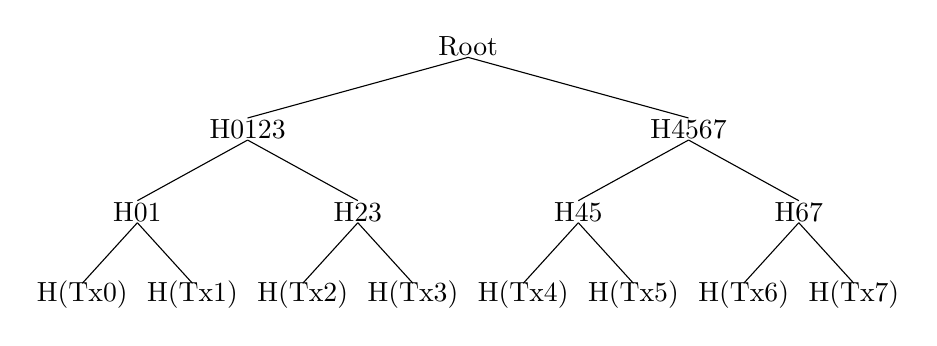
\begin{tikzpicture}[scale=0.7]
			% Leaf nodes
			\node at (0,0) {H(Tx0)};
			\node at (2,0) {H(Tx1)};
			\node at (4,0) {H(Tx2)};
			\node at (6,0) {H(Tx3)};
			\node at (8,0) {H(Tx4)};
			\node at (10,0) {H(Tx5)};
			\node at (12,0) {H(Tx6)};
			\node at (14,0) {H(Tx7)};

			% Level 1
			\node at (1,1.5) {H01};
			\node at (5,1.5) {H23};
			\node at (9,1.5) {H45};
			\node at (13,1.5) {H67};

			% Level 2
			\node at (3,3) {H0123};
			\node at (11,3) {H4567};

			% Root
			\node at (7,4.5) {Root};

			% Draw edges
			\draw (0,0.2) -- (1,1.3);
			\draw (2,0.2) -- (1,1.3);
			\draw (4,0.2) -- (5,1.3);
			\draw (6,0.2) -- (5,1.3);
			\draw (8,0.2) -- (9,1.3);
			\draw (10,0.2) -- (9,1.3);
			\draw (12,0.2) -- (13,1.3);
			\draw (14,0.2) -- (13,1.3);

			\draw (1,1.7) -- (3,2.8);
			\draw (5,1.7) -- (3,2.8);
			\draw (9,1.7) -- (11,2.8);
			\draw (13,1.7) -- (11,2.8);

			\draw (3,3.2) -- (7,4.3);
			\draw (11,3.2) -- (7,4.3);
		\end{tikzpicture}
	\end{center}
\end{frame}

\begin{frame}{Merkle trees in Bitcoin blocks}
	\begin{itemize}
		\item Each Bitcoin block header contains:
		      \begin{itemize}
			      \item Version number
			      \item Previous block hash
			      \item Merkle root of all transactions
			      \item Timestamp
			      \item Difficulty target
			      \item Nonce
		      \end{itemize}
		\item Block header is only 80 bytes.
		\item Merkle root represents all transactions in just 32 bytes.
	\end{itemize}
\end{frame}

\begin{frame}{Why use Merkle trees?}
	\begin{itemize}
		\item \textbf{Efficiency}: Verify transaction inclusion without full block.
		\item \textbf{Security}: Any change to transactions changes root.
		\item \textbf{Scalability}: Enables light clients (SPV wallets).
		\item \textbf{Privacy}: Can prove inclusion without revealing all transactions.
		\item \textbf{Storage}: Nodes can prune verified transactions, keep only headers.
	\end{itemize}
\end{frame}

\begin{frame}{Merkle proofs}
	\begin{itemize}
		\item To prove a transaction is in a block:
		      \begin{enumerate}
			      \item Provide the transaction.
			      \item Provide ``authentication path'' (sibling hashes).
			      \item Verifier recomputes hashes up to root.
			      \item Compare with known Merkle root.
		      \end{enumerate}
		\item Path length: $\log_2(n)$ for $n$ transactions.
		\item Example: 1000 transactions need only \approx10 hashes.
	\end{itemize}
\end{frame}

\begin{frame}{Merkle proof example}
	\begin{itemize}
		\item Proving Tx2 is in the block:
	\end{itemize}
	\begin{center}
		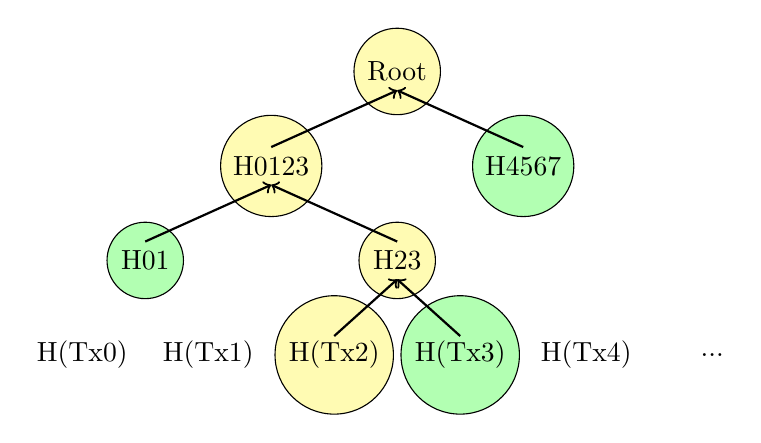
\begin{tikzpicture}[scale=0.8]
			% Highlight path
			\node[draw,circle,fill=yellow!30] at (4,0) {H(Tx2)};
			\node[draw,circle,fill=green!30] at (6,0) {H(Tx3)};
			\node[draw,circle,fill=yellow!30] at (5,1.5) {H23};
			\node[draw,circle,fill=green!30] at (1,1.5) {H01};
			\node[draw,circle,fill=yellow!30] at (3,3) {H0123};
			\node[draw,circle,fill=green!30] at (7,3) {H4567};
			\node[draw,circle,fill=yellow!30] at (5,4.5) {Root};

			% Other nodes
			\node at (0,0) {H(Tx0)};
			\node at (2,0) {H(Tx1)};
			\node at (8,0) {H(Tx4)};
			\node at (10,0) {...};

			% Draw relevant edges
			\draw[thick,->] (4,0.3) -- (5,1.2);
			\draw[thick,->] (6,0.3) -- (5,1.2);
			\draw[thick,->] (5,1.8) -- (3,2.7);
			\draw[thick,->] (1,1.8) -- (3,2.7);
			\draw[thick,->] (3,3.3) -- (5,4.2);
			\draw[thick,->] (7,3.3) -- (5,4.2);
		\end{tikzpicture}
	\end{center}
	\begin{itemize}
		\item Need: H(Tx2), H(Tx3), H01, H4567
	\end{itemize}
\end{frame}

\begin{frame}{Verification process}
	\begin{itemize}
		\item Given: Transaction Tx2 and proof [H(Tx3), H01, H4567]
		\item Verification steps:
		      \begin{enumerate}
			      \item Compute \func{hash}{Tx2}
			      \item Compute H23 = \func{hash}{\func{hash}{Tx2} \| H(Tx3)}
			      \item Compute H0123 = \func{hash}{H01 \| H23}
			      \item Compute Root = \func{hash}{H0123 \| H4567}
			      \item Check if computed root matches block header
		      \end{enumerate}
		\item Total data needed: \approx100 bytes instead of entire block (\approx1MB)
	\end{itemize}
\end{frame}

\begin{frame}{SPV (Simplified Payment Verification)}
	\begin{itemize}
		\item Satoshi's solution for lightweight clients.
		\item SPV clients only download:
		      \begin{itemize}
			      \item Block headers (80 bytes each)
			      \item Merkle proofs for relevant transactions
		      \end{itemize}
		\item Storage requirement:
		      \begin{itemize}
			      \item Full node: \approx500GB (all transactions)
			      \item SPV client: \approx60MB (headers only)
		      \end{itemize}
		\item Trade-off: Trust that longest chain is valid.
	\end{itemize}
\end{frame}

\begin{frame}{Handling odd numbers of transactions}
	\begin{itemize}
		\item Merkle trees need even number of nodes at each level.
		\item Bitcoin's solution: Duplicate the last transaction if odd.
		\item Example with 5 transactions:
		      \begin{itemize}
			      \item Leaves: H(Tx0), H(Tx1), H(Tx2), H(Tx3), H(Tx4), H(Tx4)
			      \item Note: Tx4 hash is duplicated
		      \end{itemize}
		\item This ensures tree is always complete.
		\item Important: Duplicate the hash, not the transaction.
	\end{itemize}
\end{frame}

\begin{frame}{Security properties}
	\begin{itemize}
		\item \textbf{Tamper evidence}: Changing any transaction changes root.
		\item \textbf{Collision resistance}: Inherits from underlying hash function.
		\item \textbf{Second preimage resistance}: Can't find different transaction with same Merkle path.
		\item \textbf{Commitment}: Root commits to all transactions and their order.
	\end{itemize}
\end{frame}

\begin{frame}{Merkle tree attacks and defenses}
	\begin{itemize}
		\item \textbf{Potential attack}: Malicious miner includes invalid transaction.
		\item SPV clients can't detect without validating transaction.
		\item \textbf{Defense}: Economic incentives
		      \begin{itemize}
			      \item Invalid blocks rejected by full nodes.
			      \item Miner loses block reward.
			      \item Requires majority of miners to collude.
		      \end{itemize}
		\item \textbf{Best practice}: SPV clients should connect to multiple nodes.
	\end{itemize}
\end{frame}

\begin{frame}{Future improvements}
	\begin{itemize}
		\item \textbf{UTXO commitments}: Merkle tree of unspent outputs.
		\item \textbf{Fraud proofs}: Compact proofs of invalid transactions.
		\item \textbf{Merkle-sum trees}: Include transaction amounts in tree.
		\item \textbf{Alternative structures}:
		      \begin{itemize}
			      \item Verkle trees (more efficient proofs)
			      \item Sparse Merkle trees (better for state)
		      \end{itemize}
	\end{itemize}
\end{frame}

\begin{frame}{Merkle trees beyond Bitcoin}
	\begin{itemize}
		\item Used extensively in other cryptocurrencies:
		      \begin{itemize}
			      \item Ethereum: State tree, transaction tree, receipt tree
			      \item Certificate Transparency: Merkle tree of SSL certificates
			      \item Git: Similar structure for version control
			      \item IPFS: Content-addressed storage
			      \item MLS (TreeKEM): As seen in our Secure Messaging topic!
		      \end{itemize}
		\item Key primitive for authenticated data structures.
		\item Enables efficient cryptographic commitments at scale.
	\end{itemize}
\end{frame}

\section{Ethereum, Smart Contracts and Layer 2s}

\begin{frame}{Beyond digital cash: The limitations of Bitcoin}
	\begin{itemize}
		\item Bitcoin solved digital cash, but is intentionally limited:
		      \begin{itemize}
			      \item Script language is not Turing-complete
			      \item Can only express simple spending conditions
			      \item No loops, limited opcodes, minimal state
		      \end{itemize}
		\item What if we could do more than just payments?
		      \begin{itemize}
			      \item Financial contracts (loans, derivatives, escrow)
			      \item Decentralized organizations (DAOs)
			      \item Digital property rights
			      \item Programmable money with complex logic
		      \end{itemize}
	\end{itemize}
\end{frame}

\begin{frame}{Ethereum: A world computer}
	\begin{itemize}
		\item Proposed by Vitalik Buterin and friends
		\item Core insight: Blockchain + Turing-complete programming
		      \begin{itemize}
			      \item The blockchain would store virtual machine instructions that nodes would execute!
			      \item These VM instructions would be compiled from a Turing-complete programming language.
			      \item We call them ``smart contracts''.
		      \end{itemize}
		\item Vision: ``World computer'' that can execute any computation
		\item Key properties:
		      \begin{itemize}
			      \item Decentralized like Bitcoin
			      \item But programmable with arbitrary logic
			      \item Global shared state machine
			      \item Trustless code execution
		      \end{itemize}
	\end{itemize}
\end{frame}

\begin{frame}{From transactions to state transitions}
	\begin{itemize}
		\item Bitcoin: Transaction-based ledger
		      \begin{itemize}
			      \item Tracks coin ownership via UTXO model
			      \item Transactions consume and create outputs
			      \item Limited scripting for spending conditions
		      \end{itemize}
		\item Ethereum: Account-based state machine
		      \begin{itemize}
			      \item Every address has a state (balance, code, storage)
			      \item Transactions trigger state transitions
			      \item State transitions can execute arbitrary code
			      \item Result: Programmable blockchain
		      \end{itemize}
	\end{itemize}
\end{frame}

\begin{frame}{The Ethereum Virtual Machine (EVM)}
	\begin{itemize}
		\item Decentralized computation engine
		\item Properties:
		      \begin{itemize}
			      \item Stack-based virtual machine
			      \item 256-bit word size (matches cryptographic operations)
			      \item Deterministic execution (same input \rightarrow\ same output)
			      \item Isolated sandbox environment
		      \end{itemize}
		\item Every node runs the EVM:
		      \begin{itemize}
			      \item Executes smart contract code
			      \item Updates global state
			      \item Ensures consensus on computation results
		      \end{itemize}
	\end{itemize}
\end{frame}

\begin{frame}{Accounts in Ethereum}
	\begin{itemize}
		\item Two types of accounts:
		      \begin{itemize}
			      \item \textbf{Externally Owned Accounts (EOAs)}:
			            \begin{itemize}
				            \item Controlled by private keys
				            \item Can initiate transactions
				            \item Like Bitcoin addresses
			            \end{itemize}
			      \item \textbf{Contract Accounts}:
			            \begin{itemize}
				            \item Controlled by code
				            \item Have associated bytecode
				            \item Can store persistent data
				            \item Can't initiate transactions
			            \end{itemize}
		      \end{itemize}
		\item Both can hold ETH and interact with other accounts
	\end{itemize}
\end{frame}

\begin{frame}{The gas mechanism}
	\begin{itemize}
		\item Problem: How to prevent infinite loops and spam?
		\item Solution: ``Gas'' - computational fuel
		\item How it works:
		      \begin{itemize}
			      \item Every operation costs gas (ADD: 3, MUL: 5, SSTORE: 20,000)
			      \item Users specify gas limit and gas price
			      \item Transaction fee = gas used × gas price
			      \item If gas runs out, transaction reverts
		      \end{itemize}
		\item Benefits:
		      \begin{itemize}
			      \item Halting problem solved economically
			      \item DoS protection
			      \item Fair resource pricing
		      \end{itemize}
	\end{itemize}
\end{frame}

\begin{frame}{State storage in Ethereum}
	\begin{itemize}
		\item Each account has:
		      \begin{itemize}
			      \item \textbf{Nonce}: Transaction counter (replay protection)
			      \item \textbf{Balance}: Amount of ETH
			      \item \textbf{Code}: Contract bytecode (if contract account)
			      \item \textbf{Storage}: Key-value store (if contract account)
		      \end{itemize}
		\item Storage is persistent:
		      \begin{itemize}
			      \item Survives between transactions
			      \item 256-bit keys \rightarrow\ 256-bit values
			      \item Expensive to write (20,000 gas)
			      \item Cheap to read (200 gas)
		      \end{itemize}
	\end{itemize}
\end{frame}

\begin{frame}{Ethereum's Merkle Patricia Trie}
	\begin{itemize}
		\item Bitcoin uses Merkle trees for transactions only
		\item Ethereum needs to store entire state efficiently
		\item Solution: Modified Merkle Patricia Trie
		      \begin{itemize}
			      \item Combines trie structure with Merkle proofs
			      \item Efficient updates (only change affected path)
			      \item Compact storage (shared prefixes)
			      \item Cryptographic proofs of state
		      \end{itemize}
		\item Enables light clients to verify account states
	\end{itemize}
\end{frame}

\begin{frame}{Transaction types in Ethereum}
	\begin{itemize}
		\item \textbf{Simple transfer}: Send ETH between accounts
		\item \textbf{Contract creation}: Deploy new smart contract
		      \begin{itemize}
			      \item Transaction data contains contract bytecode
			      \item Creates new contract account at computed address
		      \end{itemize}
		\item \textbf{Contract interaction}: Call smart contract function
		      \begin{itemize}
			      \item Transaction data contains function selector + arguments
			      \item Triggers code execution in EVM
		      \end{itemize}
		\item All require gas and can transfer ETH
	\end{itemize}
\end{frame}

\begin{frame}{The blockchain trilemma}
	\begin{itemize}
		\item Three desirable properties:
		      \begin{itemize}
			      \item \textbf{Decentralization}: Many independent validators
			      \item \textbf{Security}: Resistant to attacks
			      \item \textbf{Scalability}: High transaction throughput
		      \end{itemize}
		\item The trilemma: Hard to achieve all three
		\item Bitcoin's choice: Decentralization + Security
		\item Early Ethereum: Same choice, but worse scalability
		      \begin{itemize}
			      \item More complex state transitions
			      \item Larger state size
			      \item Result: \approx15 transactions per second
		      \end{itemize}
	\end{itemize}
\end{frame}

\begin{frame}{Ethereum's evolution: From PoW to PoS}
	\begin{itemize}
		\item Originally used Proof-of-Work like Bitcoin
		\item September 2022: ``The Merge'' to Proof-of-Stake
		\item Proof-of-Stake mechanism:
		      \begin{itemize}
			      \item Validators ``stake'' 32 ETH as collateral
			      \item Selected randomly to propose blocks
			      \item Misbehavior results in ``slashing'' (losing stake)
			      \item No mining, drastically lower energy use
		      \end{itemize}
		\item Benefits:
		      \begin{itemize}
			      \item 99.95\% reduction in energy consumption
			      \item Better finality guarantees
			      \item Foundation for future scaling
		      \end{itemize}
	\end{itemize}
\end{frame}

\begin{frame}{Why Ethereum matters}
	\begin{itemize}
		\item Enabled entirely new applications:
		      \begin{itemize}
			      \item \textbf{DeFi}: Decentralized finance (\approx\$50B locked)
			      \item \textbf{NFTs}: Digital ownership and art (depending on your perspective)
			      \item \textbf{DAOs}: Decentralized autonomous organizations
			      \item \textbf{Stablecoins}: Crypto-native stable currencies
		      \end{itemize}
		\item Inspired countless innovations:
		      \begin{itemize}
			      \item Alternative Layer 1 blockchains
			      \item Layer 2 scaling solutions
			      \item Cross-chain bridges
			      \item Zero-knowledge applications
		      \end{itemize}
		\item Created a platform for permissionless innovation
	\end{itemize}
\end{frame}

\subsection{Proof of Stake}

\begin{frame}{What is Proof of Stake?}
	\begin{itemize}
		\item Alternative consensus mechanism to Proof of Work
		\item Instead of computational power, uses economic stake
		\item Core concept:
		      \begin{itemize}
			      \item Validators lock up cryptocurrency as collateral
			      \item Selected to create blocks based on stake size
			      \item Misbehavior punished by losing stake (``slashing'')
			      \item No mining or energy-intensive computations
		      \end{itemize}
		\item ``Skin in the game'' security model
	\end{itemize}
\end{frame}

\begin{frame}{How Proof of Stake works}
	\begin{itemize}
		\item \textbf{Becoming a validator}:
		      \begin{itemize}
			      \item Deposit required stake (32 ETH for Ethereum)
			      \item Run validator software
			      \item Stay online and participate honestly
		      \end{itemize}
		\item \textbf{Block production}:
		      \begin{itemize}
			      \item Validators randomly selected to propose blocks
			      \item Selection weighted by stake amount
			      \item Other validators attest to block validity
			      \item Consensus reached through attestations
		      \end{itemize}
	\end{itemize}
\end{frame}

\begin{frame}{Ethereum's long road to PoS}
	\begin{itemize}
		\item 2014: PoS mentioned in Ethereum whitepaper
		\item 2015-2020: Research and development
		      \begin{itemize}
			      \item Solving ``nothing at stake'' problem
			      \item Designing slashing conditions
			      \item Finality mechanisms (Casper FFG)
			      \item Fork choice rules (LMD-GHOST)
		      \end{itemize}
		\item December 2020: Beacon Chain launches
		      \begin{itemize}
			      \item PoS chain running parallel to PoW
			      \item Validators start staking
			      \item No transactions yet, just consensus
		      \end{itemize}
	\end{itemize}
\end{frame}

\begin{frame}{The Merge: Technical achievement}
	\begin{itemize}
		\item September 15, 2022: The Merge executed
		\item Unprecedented technical feat:
		      \begin{itemize}
			      \item Swapped consensus engine while running
			      \item Like ``changing jet engine mid-flight''
			      \item Zero downtime
			      \item \$200B+ value at stake
		      \end{itemize}
		\item Two chains became one:
		      \begin{itemize}
			      \item Execution layer (former PoW chain)
			      \item Consensus layer (Beacon Chain)
			      \item Seamless transition at block 15,537,394
		      \end{itemize}
	\end{itemize}
\end{frame}

\begin{frame}{Why the switch mattered: Environmental impact}
	\begin{itemize}
		\item \textbf{Energy reduction}: 99.95\% decrease
		      \begin{itemize}
			      \item Before: \approx78 TWh/year (Austria's consumption)
			      \item After: \approx0.01 TWh/year
			      \item From 13,000 US households to 10 households equivalent
		      \end{itemize}
		\item \textbf{Carbon footprint}:
		      \begin{itemize}
			      \item Eliminated \approx11 million tons CO2/year
			      \item Equivalent to removing 2.4 million cars
		      \end{itemize}
		\item Made Ethereum environmentally sustainable
	\end{itemize}
\end{frame}

\begin{frame}{Why the switch mattered: Security model}
	\begin{itemize}
		\item \textbf{Economic security}:
		      \begin{itemize}
			      \item \approx\$40B worth of ETH staked
			      \item Attack cost: Need 51\% of stake
			      \item Attackers lose their stake if caught
		      \end{itemize}
		\item \textbf{Better finality}:
		      \begin{itemize}
			      \item Blocks become ``finalized'' after 2 epochs (\approx13 minutes)
			      \item Finalized blocks cannot be reverted
			      \item Stronger guarantees than probabilistic PoW finality
		      \end{itemize}
		\item \textbf{Slashing conditions}:
		      \begin{itemize}
			      \item Double signing: Lose stake
			      \item Being offline: Gradual penalties
			      \item Censorship: Future slashing conditions planned
		      \end{itemize}
	\end{itemize}
\end{frame}

\begin{frame}{Validator economics}
	\begin{itemize}
		\item \textbf{Rewards}:
		      \begin{itemize}
			      \item Block proposals: \approx0.05 ETH per block
			      \item Attestations: Small continuous rewards
			      \item MEV tips: Additional profits from transaction ordering
			      \item Annual yield: \approx4-5\% currently
		      \end{itemize}
		\item \textbf{Penalties}:
		      \begin{itemize}
			      \item Offline penalties: Small, proportional to downtime
			      \item Slashing: 1 ETH minimum + ejection
			      \item Correlated slashing: Up to 100\% of stake
		      \end{itemize}
	\end{itemize}
\end{frame}

\begin{frame}{Results: Network statistics}
	\begin{itemize}
		\item \textbf{Validator participation}:
		      \begin{itemize}
			      \item Over 900,000 active validators
			      \item \approx30 million ETH staked (25\% of supply)
			      \item Distributed across 7,000+ unique entities
			      \item 99.9\%+ network uptime maintained
		      \end{itemize}
		\item \textbf{Performance improvements}:
		      \begin{itemize}
			      \item Block time: Consistent 12 seconds
			      \item Finality: 13 minutes (vs never in PoW)
			      \item Predictable block production
			      \item Lower fee volatility
		      \end{itemize}
	\end{itemize}
\end{frame}

\begin{frame}{Results: Ecosystem impact}
	\begin{itemize}
		\item \textbf{Staking services emerged}:
		      \begin{itemize}
			      \item Liquid staking protocols (Lido, Rocket Pool)
			      \item Institutional staking services
			      \item Distributed validator technology
		      \end{itemize}
		\item \textbf{New economic dynamics}:
		      \begin{itemize}
			      \item ETH became yield-bearing asset
			      \item Staking derivatives (stETH) as DeFi collateral
			      \item MEV markets formalized
		      \end{itemize}
		\item \textbf{Development velocity}:
		      \begin{itemize}
			      \item Faster protocol upgrades possible
			      \item Foundation for future scaling (sharding)
		      \end{itemize}
	\end{itemize}
\end{frame}

\begin{frame}{Criticisms and trade-offs}
	\begin{itemize}
		\item \textbf{Centralization concerns}:
		      \begin{itemize}
			      \item 32 ETH requirement excludes many users
			      \item Liquid staking protocols control large stakes
			      \item Economies of scale favor large operators
		      \end{itemize}
		\item \textbf{Complexity}:
		      \begin{itemize}
			      \item More complex than PoW conceptually
			      \item Harder to reason about security
			      \item Requires active participation
		      \end{itemize}
		\item \textbf{New attack vectors}:
		      \begin{itemize}
			      \item MEV exploitation
			      \item Stake grinding attacks
			      \item Social layer attacks
		      \end{itemize}
	\end{itemize}
\end{frame}

\begin{frame}{Future developments}
	\begin{itemize}
		\item \textbf{Protocol improvements}:
		      \begin{itemize}
			      \item Single slot finality (seconds vs minutes)
			      \item Distributed validator technology standard
			      \item Anti-correlation penalties
			      \item Secret leader election
		      \end{itemize}
		\item \textbf{Scaling benefits}:
		      \begin{itemize}
			      \item Enables data availability sampling
			      \item Foundation for sharding
			      \item Better light client support
		      \end{itemize}
		\item \textbf{Broader adoption}:
		      \begin{itemize}
			      \item Many chains following Ethereum's lead
			      \item PoS becoming dominant consensus mechanism
		      \end{itemize}
	\end{itemize}
\end{frame}

\subsection{Smart Contracts}

\begin{frame}{What are smart contracts?}
	\begin{itemize}
		\item Self-executing code deployed on blockchain
		\item Key properties:
		      \begin{itemize}
			      \item \textbf{Immutable}: Code cannot be changed after deployment
			      \item \textbf{Deterministic}: Same input always produces same output
			      \item \textbf{Autonomous}: Execute without intermediaries
			      \item \textbf{Transparent}: Code is public and verifiable
		      \end{itemize}
		\item Not really ``smart'' or legal ``contracts''
		      \begin{itemize}
			      \item Better term: Persistent scripts
			      \item But ``smart contracts'' name stuck
		      \end{itemize}
	\end{itemize}
\end{frame}

\begin{frame}{From vending machines to world computer}
	\begin{itemize}
		\item Nick Szabo's vending machine analogy (1997):
		      \begin{itemize}
			      \item Insert coin \rightarrow\ get product
			      \item No human intermediary needed
			      \item Rules encoded in mechanism
		      \end{itemize}
		\item Smart contracts extend this concept:
		      \begin{itemize}
			      \item Arbitrary complex logic
			      \item Multiple parties
			      \item Conditional execution
			      \item Automatic enforcement
		      \end{itemize}
		\item Examples: Escrow, auctions, loans, insurance, governance
	\end{itemize}
\end{frame}

\begin{frame}{How smart contracts work}
	\begin{itemize}
		\item \textbf{Deployment}:
		      \begin{enumerate}
			      \item Write contract code (usually Solidity)
			      \item Compile to EVM bytecode
			      \item Send deployment transaction
			      \item Contract gets unique address
		      \end{enumerate}
		\item \textbf{Interaction}:
		      \begin{enumerate}
			      \item Users send transactions to contract address
			      \item Transaction includes function call + parameters
			      \item All nodes execute the code
			      \item State changes recorded on blockchain
		      \end{enumerate}
	\end{itemize}
\end{frame}

\begin{frame}{Contract lifecycle}
	\begin{itemize}
		\item \textbf{Birth}: Contract deployed to blockchain
		      \begin{itemize}
			      \item Constructor runs once
			      \item Initial state set
			      \item Address determined by deployer + nonce
		      \end{itemize}
		\item \textbf{Life}: Users interact with contract
		      \begin{itemize}
			      \item Functions called via transactions
			      \item State updated
			      \item Events emitted
		      \end{itemize}
		\item \textbf{Death} (optional): Contract self-destructs
		      \begin{itemize}
			      \item \texttt{selfdestruct} opcode (deprecated)
			      \item Sends remaining ETH to specified address
			      \item Contract code removed
		      \end{itemize}
	\end{itemize}
\end{frame}

\begin{frame}{Solidity: The language of smart contracts}
	\begin{itemize}
		\item High-level language for EVM
		\item Created by Gavin Wood (Ethereum co-founder)
		\item Design influences:
		      \begin{itemize}
			      \item JavaScript (syntax)
			      \item C++ (types)
			      \item Python (modifiers)
		      \end{itemize}
		\item Statically typed, supports:
		      \begin{itemize}
			      \item Inheritance
			      \item Libraries
			      \item Complex types
			      \item Inline assembly
		      \end{itemize}
	\end{itemize}
\end{frame}

\begin{frame}[fragile]{Your first smart contract}
	\begin{verbatim}
pragma solidity ^0.8.0;
contract SimpleStorage {
    uint256 public storedNumber;
    function store(uint256 _number) public {
        storedNumber = _number;
    }
    function retrieve() public view returns (uint256) {
        return storedNumber;
    }
}
 \end{verbatim}
\end{frame}

\begin{frame}{Anatomy of a Solidity contract}
	\begin{itemize}
		\item \textbf{Pragma}: Compiler version requirement
		\item \textbf{Contract keyword}: Defines contract scope
		\item \textbf{State variables}: Persistent storage
		\item \textbf{Functions}: Contract behavior
		\item \textbf{Visibility modifiers}:
		      \begin{itemize}
			      \item \texttt{public}: Callable by anyone
			      \item \texttt{private}: Only within contract
			      \item \texttt{internal}: Within contract + inherited
			      \item \texttt{external}: Only from outside
		      \end{itemize}
	\end{itemize}
\end{frame}

\begin{frame}{State mutability and gas optimization}
	\begin{itemize}
		\item Function modifiers indicate state access:
		      \begin{itemize}
			      \item \texttt{view}: Reads state, no modifications
			      \item \texttt{pure}: No state access at all
			      \item (default): Can modify state
		      \end{itemize}
		\item Why this matters:
		      \begin{itemize}
			      \item \texttt{view}/\texttt{pure} functions free when called externally
			      \item State modifications cost gas
			      \item Compiler can optimize based on mutability
		      \end{itemize}
		\item Best practice: Use most restrictive modifier possible
	\end{itemize}
\end{frame}

\begin{frame}[fragile]{A more realistic example: Simple token}
	\scriptsize
	\begin{verbatim}
contract SimpleToken {
    mapping(address => uint256) public balances;
    uint256 public totalSupply;

    constructor(uint256 _initialSupply) {
        balances[msg.sender] = _initialSupply;
        totalSupply = _initialSupply;
    }

    function transfer(address _to, uint256 _amount)
        public returns (bool) {
        require(balances[msg.sender] >= _amount);
        balances[msg.sender] -= _amount;
        balances[_to] += _amount;
        return true;
    }
}
\end{verbatim}
\end{frame}

\begin{frame}{Key Solidity concepts}
	\begin{itemize}
		\item \textbf{\texttt{msg.sender}}: Address calling the function
		\item \textbf{Mappings}: Key-value storage (like hash tables)
		\item \textbf{Constructor}: Runs once at deployment
		\item \textbf{\texttt{require()}}: Reverts transaction if condition false
		\item \textbf{State changes}: Automatic and persistent
		\item Transaction atomicity: All or nothing execution
	\end{itemize}
\end{frame}

\begin{frame}{The magic of \texttt{msg.sender}}
	\begin{itemize}
		\item Every function call has context:
		      \begin{itemize}
			      \item \texttt{msg.sender}: Who called this function
			      \item \texttt{msg.value}: ETH sent with call
			      \item \texttt{msg.data}: Complete calldata
			      \item \texttt{block.timestamp}: Current block time
			      \item \texttt{block.number}: Current block height
		      \end{itemize}
		\item This enables:
		      \begin{itemize}
			      \item Authentication without passwords
			      \item Payment handling
			      \item Time-based logic
			      \item Access control
		      \end{itemize}
	\end{itemize}
\end{frame}

\begin{frame}[fragile]{Events: The blockchain's logs}
	\begin{itemize}
		\item Smart contracts can emit events:
		      \begin{itemize}
			      \item Cheap way to store data (not in state)
			      \item Searchable and filterable
			      \item Used by dApps to track activity
		      \end{itemize}
		\item Example:
		      \begin{verbatim}
event Transfer(address indexed from,
               address indexed to,
               uint256 value);

emit Transfer(msg.sender, _to, _amount);
        \end{verbatim}
		\item \texttt{indexed} parameters can be searched efficiently
	\end{itemize}
\end{frame}

\begin{frame}{Contract interactions}
	\begin{itemize}
		\item Contracts can call other contracts:
		      \begin{itemize}
			      \item Direct calls: \texttt{otherContract.function()}
			      \item Low-level calls: \texttt{address.call()}
			      \item Delegate calls: \texttt{address.delegatecall()}
			      \item Static calls: \texttt{address.staticcall()}
		      \end{itemize}
		\item Creates composability:
		      \begin{itemize}
			      \item DeFi ``money legos''
			      \item Protocols built on protocols
			      \item Complex interactions possible
		      \end{itemize}
		\item But also security risks...
	\end{itemize}
\end{frame}

\begin{frame}{Smart contract security: The DAO hack}
	\begin{itemize}
		\item June 2016: The DAO (Decentralized Autonomous Organization)
		\item Raised \$150M worth of ETH
		\item Reentrancy vulnerability exploited:
		      \begin{enumerate}
			      \item Attacker calls withdraw function
			      \item Contract sends ETH before updating balance
			      \item Receiving contract calls back into withdraw
			      \item Balance not yet updated, withdrawal succeeds again
			      \item Repeat until drained
		      \end{enumerate}
		\item Result: \$60M stolen, Ethereum hard fork
	\end{itemize}
\end{frame}

\begin{frame}[fragile]{Reentrancy vulnerability example}
	\begin{verbatim}
// VULNERABLE CODE - DO NOT USE
contract Vulnerable {
    mapping(address => uint) balances;
    function withdraw() public {
        uint balance = balances[msg.sender];
        // External call BEFORE state update
        (bool success,) = msg.sender.call{value: balance}("");
        require(success);
        // State update happens AFTER external call
        balances[msg.sender] = 0;
    }
}
 \end{verbatim}
\end{frame}

\begin{frame}{Common smart contract vulnerabilities}
	\begin{itemize}
		\item \textbf{Reentrancy}: External calls before state updates
		\item \textbf{Integer overflow/underflow}: Fixed in Solidity 0.8+
		\item \textbf{Access control}: Missing permission checks
		\item \textbf{Front-running}: Transaction order manipulation
		\item \textbf{Gas griefing}: Forcing out-of-gas errors
		\item \textbf{Timestamp dependence}: Miners can manipulate
		\item \textbf{Unchecked return values}: Silent failures
	\end{itemize}
\end{frame}

\begin{frame}{Security best practices}
	\begin{itemize}
		\item \textbf{Checks-Effects-Interactions pattern}:
		      \begin{enumerate}
			      \item Check conditions (require statements)
			      \item Update state (effects)
			      \item External calls (interactions) last
		      \end{enumerate}
		\item \textbf{Use established patterns}:
		      \begin{itemize}
			      \item OpenZeppelin contracts
			      \item Pull over push payments
			      \item Reentrancy guards
		      \end{itemize}
		\item \textbf{Testing and auditing}:
		      \begin{itemize}
			      \item Comprehensive test suites
			      \item Formal verification
			      \item Professional audits
			      \item Bug bounties
		      \end{itemize}
	\end{itemize}
\end{frame}

\begin{frame}{The immutability dilemma}
	\begin{itemize}
		\item Code is law... but what if code has bugs?
		\item Upgradeability patterns emerged:
		      \begin{itemize}
			      \item \textbf{Proxy patterns}: Logic/storage separation
			      \item \textbf{Diamond pattern}: Multiple implementation contracts
			      \item \textbf{Create2}: Deterministic addresses
		      \end{itemize}
		\item Trade-offs:
		      \begin{itemize}
			      \item Upgradeable = centralization risk
			      \item Immutable = can't fix bugs
			      \item Timelock = compromise solution
		      \end{itemize}
		\item Community debate continues...
	\end{itemize}
\end{frame}

\begin{frame}{Gas optimization techniques}
	\begin{itemize}
		\item Storage is expensive (20,000 gas to store)
		      \begin{itemize}
			      \item Pack structs efficiently
			      \item Use events for logs, not storage
			      \item Delete unused storage
		      \end{itemize}
		\item Computation tips:
		      \begin{itemize}
			      \item Use \texttt{unchecked} blocks when safe
			      \item Short-circuit conditions
			      \item Batch operations
		      \end{itemize}
		\item Design patterns:
		      \begin{itemize}
			      \item Merkle proofs instead of storing lists
			      \item IPFS for large data
			      \item Off-chain computation, on-chain verification
		      \end{itemize}
	\end{itemize}
\end{frame}

\begin{frame}{Real-world smart contract applications}
	\begin{itemize}
		\item \textbf{DeFi protocols}:
		      \begin{itemize}
			      \item Uniswap: Automated market maker
			      \item Aave: Lending and borrowing
			      \item MakerDAO: Stablecoin system
		      \end{itemize}
		\item \textbf{NFT standards}:
		      \begin{itemize}
			      \item ERC-721: Non-fungible tokens
			      \item ERC-1155: Multi-token standard
		      \end{itemize}
		\item \textbf{Infrastructure}:
		      \begin{itemize}
			      \item ENS: Ethereum Name Service
			      \item Gnosis Safe: Multi-signature wallets
			      \item Chainlink: Oracle networks
		      \end{itemize}
	\end{itemize}
\end{frame}

\begin{frame}{Development tools and ecosystem}
	\begin{itemize}
		\item \textbf{Development frameworks}:
		      \begin{itemize}
			      \item Hardhat: Testing and deployment
			      \item Foundry: Fast, Rust-based toolkit
			      \item Truffle: Original framework
		      \end{itemize}
		\item \textbf{Testing tools}:
		      \begin{itemize}
			      \item Fuzzing frameworks
			      \item Property-based testing
			      \item Fork testing against mainnet
		      \end{itemize}
		\item \textbf{Security tools}:
		      \begin{itemize}
			      \item Slither: Static analysis
			      \item Mythril: Symbolic execution
			      \item Echidna: Smart fuzzer
		      \end{itemize}
	\end{itemize}
\end{frame}

\begin{frame}{The future of smart contracts}
	\begin{itemize}
		\item \textbf{Language evolution}:
		      \begin{itemize}
			      \item Move (Aptos/Sui): Resource-oriented
			      \item Vyper: Python-like, security-focused
			      \item Fe: Rust-inspired for EVM
			      \item Cairo: For STARK-based systems
		      \end{itemize}
		\item \textbf{Cross-chain contracts}:
		      \begin{itemize}
			      \item Bridge protocols
			      \item Interoperability standards
			      \item Multi-chain applications
		      \end{itemize}
		\item \textbf{Zero-knowledge integration}:
		      \begin{itemize}
			      \item Private smart contracts
			      \item Efficient verification
			      \item New application possibilities
		      \end{itemize}
	\end{itemize}
\end{frame}

\subsection{Layer 1s vs. Layer 2s}

\begin{frame}{The scaling problem}
	\begin{itemize}
		\item Ethereum processes \approx15 transactions per second
		\item Visa processes \approx65,000 transactions per second
		\item The gap: 4,000x
		\item Why so slow?
		      \begin{itemize}
			      \item Every node processes every transaction
			      \item Every node stores entire state
			      \item Decentralization requires broad participation
			      \item Can't just use bigger servers
		      \end{itemize}
	\end{itemize}
\end{frame}

\begin{frame}{Layer 1 vs Layer 2: Definitions}
	\begin{itemize}
		\item \textbf{Layer 1 (L1)}: The base blockchain
		      \begin{itemize}
			      \item Bitcoin, Ethereum mainnet
			      \item Handles consensus and security
			      \item Final settlement layer
			      \item Limited throughput by design
		      \end{itemize}
		\item \textbf{Layer 2 (L2)}: Built on top of L1
		      \begin{itemize}
			      \item Inherits security from L1
			      \item Processes transactions off-chain
			      \item Periodically settles to L1
			      \item Can achieve much higher throughput
		      \end{itemize}
	\end{itemize}
\end{frame}

\begin{frame}{The Layer 2 insight}
	\begin{itemize}
		\item Key realization: Not every node needs to execute every transaction
		\item Instead:
		      \begin{itemize}
			      \item Execute transactions elsewhere
			      \item Post compressed results to L1
			      \item Provide cryptographic proofs of correctness
			      \item L1 validates proofs, not transactions
		      \end{itemize}
		\item Benefits:
		      \begin{itemize}
			      \item Inherit L1 security
			      \item Dramatically lower costs
			      \item Much higher throughput
			      \item Specialized execution environments
		      \end{itemize}
	\end{itemize}
\end{frame}

\begin{frame}{Types of Layer 2 solutions}
	\begin{itemize}
		\item \textbf{State Channels}
		      \begin{itemize}
			      \item Oldest L2 concept (Lightning Network)
			      \item Off-chain transactions between fixed parties
		      \end{itemize}
		\item \textbf{Sidechains}
		      \begin{itemize}
			      \item Independent blockchains with bridges
			      \item Own consensus mechanism
		      \end{itemize}
		\item \textbf{Plasma}
		      \begin{itemize}
			      \item Child chains with fraud proofs
			      \item Largely abandoned due to UX issues
		      \end{itemize}
		\item \textbf{Rollups}
		      \begin{itemize}
			      \item Current dominant approach
			      \item Two main types: Optimistic and ZK
		      \end{itemize}
	\end{itemize}
\end{frame}

\begin{frame}{State channels: Lightning Network}
	\begin{itemize}
		\item Bitcoin's Layer 2 solution
		\item How it works:
		      \begin{itemize}
			      \item Two parties lock funds in multi-sig
			      \item Exchange signed transactions off-chain
			      \item Only final state posted to blockchain
		      \end{itemize}
		\item Advantages:
		      \begin{itemize}
			      \item Instant transactions
			      \item Minimal fees
			      \item High privacy
		      \end{itemize}
		\item Limitations:
		      \begin{itemize}
			      \item Need channel with counterparty
			      \item Capital locked in channels
			      \item Limited to payments
		      \end{itemize}
	\end{itemize}
\end{frame}

\begin{frame}{Sidechains: Polygon PoS}
	\begin{itemize}
		\item Separate blockchain with bridge to Ethereum
		\item Architecture:
		      \begin{itemize}
			      \item Own validator set (100 validators)
			      \item Modified Proof of Stake consensus
			      \item Checkpoints to Ethereum periodically
		      \end{itemize}
		\item Trade-offs:
		      \begin{itemize}
			      \item[\mycheckmark] High throughput (65,000 TPS theoretical)
			      \item[\mycheckmark] Low fees (\approx\$0.01 per transaction)
			      \item[\times] Weaker security (own validator set)
			      \item[\times] Bridge risk (wrapped assets)
		      \end{itemize}
		\item \$2B+ total value locked
	\end{itemize}
\end{frame}

\begin{frame}{The rollup revolution}
	\begin{itemize}
		\item Core idea: Computation off-chain, data on-chain
		\item All transactions posted to L1 (compressed)
		\item Anyone can reconstruct full state
		\item Two approaches to ensure correctness:
		      \begin{itemize}
			      \item \textbf{Optimistic}: Assume correct, allow challenges
			      \item \textbf{Zero-knowledge}: Provide cryptographic proofs
		      \end{itemize}
		\item Currently processing more transactions than Ethereum L1
	\end{itemize}
\end{frame}

\begin{frame}{Optimistic rollups: How they work}
	\begin{itemize}
		\item ``Optimistic'' = assume transactions are valid
		\item Fraud proof mechanism:
		      \begin{enumerate}
			      \item Sequencer posts state root to L1
			      \item 7-day challenge period
			      \item Anyone can challenge with fraud proof
			      \item If fraud proven, sequencer loses bond
		      \end{enumerate}
		\item State posted to L1 as calldata
		\item Full nodes execute all transactions
		\item Users trust either by running node or 1-of-N assumption
	\end{itemize}
\end{frame}

\begin{frame}{Optimistic rollups: Arbitrum}
	\begin{itemize}
		\item Largest optimistic rollup by TVL (\approx\$15B)
		\item Technical design:
		      \begin{itemize}
			      \item Interactive fraud proofs (multi-round)
			      \item AVM: Custom virtual machine
			      \item Nitro upgrade: WASM-based execution
		      \end{itemize}
		\item Performance:
		      \begin{itemize}
			      \item \approx40,000 TPS capacity
			      \item \approx\$0.10-0.50 per transaction
			      \item 7-day withdrawal period
		      \end{itemize}
		\item ``EVM equivalent'' - easy to port dApps
	\end{itemize}
\end{frame}

\begin{frame}{Optimistic rollups: Optimism}
	\begin{itemize}
		\item Second largest optimistic rollup (\approx\$7B TVL)
		\item Technical differences from Arbitrum:
		      \begin{itemize}
			      \item Single-round fraud proofs
			      \item Cannon: Fault proof system using MIPS
			      \item Bedrock: Modular architecture
		      \end{itemize}
		\item Innovations:
		      \begin{itemize}
			      \item OP Stack: Framework for building L2s
			      \item Superchain vision: Network of L2s
			      \item Retroactive public goods funding
		      \end{itemize}
	\end{itemize}
\end{frame}

\begin{frame}{ZK rollups: The endgame?}
	\begin{itemize}
		\item Use zero-knowledge proofs for validity
		\item Every state transition includes proof
		\item No need for challenge period
		\item Benefits:
		      \begin{itemize}
			      \item Instant finality (no 7-day wait)
			      \item Better capital efficiency
			      \item Lower long-term costs
			      \item No need to trust sequencer
		      \end{itemize}
		\item Challenges:
		      \begin{itemize}
			      \item Complex to build
			      \item Expensive to generate proofs
			      \item Harder to achieve EVM compatibility
		      \end{itemize}
	\end{itemize}
\end{frame}

\begin{frame}{ZK rollups: Technical approaches}
	\begin{itemize}
		\item Two main proof systems:
		\item \textbf{SNARKs} (Succinct Non-interactive Arguments of Knowledge)
		      \begin{itemize}
			      \item Smaller proofs (\approx200 bytes)
			      \item Requires trusted setup
			      \item Faster verification
		      \end{itemize}
		\item \textbf{STARKs} (Scalable Transparent Arguments of Knowledge)
		      \begin{itemize}
			      \item Larger proofs (\approx100 KB)
			      \item No trusted setup
			      \item Post-quantum secure
			      \item Better for complex computations
		      \end{itemize}
	\end{itemize}
\end{frame}

\begin{frame}{ZK rollup example: zkSync Era}
	\begin{itemize}
		\item First ZK rollup to achieve ``EVM compatibility''
		\item Architecture:
		      \begin{itemize}
			      \item Custom VM with different opcodes
			      \item Solidity/Vyper compiler for their VM
			      \item SNARK proofs (Plonk)
			      \item State diffs instead of transaction data
		      \end{itemize}
		\item Innovations:
		      \begin{itemize}
			      \item Account abstraction native
			      \item Paymasters (gasless transactions)
			      \item \approx2,000 TPS current capacity
		      \end{itemize}
	\end{itemize}
\end{frame}

\begin{frame}{ZK rollup example: StarkNet}
	\begin{itemize}
		\item Built by StarkWare using STARKs
		\item Unique approach:
		      \begin{itemize}
			      \item Cairo: Custom programming language
			      \item Not EVM compatible by design
			      \item Built for proof efficiency
		      \end{itemize}
		\item Features:
		      \begin{itemize}
			      \item Native account abstraction
			      \item Fractal scaling (L3s possible)
			      \item Volition: Choose between rollup/validium
		      \end{itemize}
		\item Trade-off: Better performance, harder adoption
	\end{itemize}
\end{frame}

\begin{frame}{ZK rollup example: Polygon zkEVM}
	\begin{itemize}
		\item ``True'' EVM equivalence approach
		\item Technical design:
		      \begin{itemize}
			      \item Proves actual EVM execution
			      \item No custom VM or language
			      \item Uses combination of STARK + SNARK
		      \end{itemize}
		\item Benefits:
		      \begin{itemize}
			      \item Perfect compatibility
			      \item No code changes needed
			      \item Existing tools work
		      \end{itemize}
		\item Cost: More expensive proofs
	\end{itemize}
\end{frame}

\begin{frame}{The data availability problem}
	\begin{itemize}
		\item Rollups post data to Ethereum
		\item But Ethereum calldata is expensive
		\item Cost breakdown for rollup transaction:
		      \begin{itemize}
			      \item \approx90\%: L1 data costs
			      \item \approx10\%: L2 execution costs
		      \end{itemize}
		\item Solutions emerging:
		      \begin{itemize}
			      \item EIP-4844 ``Proto-Danksharding'': Blob space
			      \item Validiums: Data off-chain
			      \item Alternative DA layers
		      \end{itemize}
	\end{itemize}
\end{frame}

\begin{frame}{Validiums and volitions}
	\begin{itemize}
		\item \textbf{Validium}: ZK rollup with off-chain data
		      \begin{itemize}
			      \item Only state root and proof on L1
			      \item Data stored elsewhere (committee, IPFS)
			      \item Much cheaper but trust assumptions
		      \end{itemize}
		\item \textbf{Volition}: User chooses data availability
		      \begin{itemize}
			      \item Rollup mode: Full security, higher cost
			      \item Validium mode: Lower security, lower cost
			      \item Same state tree, different guarantees
		      \end{itemize}
		\item Examples: StarkEx, zkPorter
	\end{itemize}
\end{frame}

\begin{frame}{Alternative data availability}
	\begin{itemize}
		\item \textbf{Celestia}: Purpose-built DA blockchain
		      \begin{itemize}
			      \item Optimized for data availability only
			      \item No execution, just ordered data
			      \item Data availability sampling
		      \end{itemize}
		\item \textbf{EigenDA}: Ethereum staker network
		      \begin{itemize}
			      \item Reuses Ethereum validator set
			      \item Slashing for data withholding
		      \end{itemize}
		\item Trade-offs:
		      \begin{itemize}
			      \item Lower cost than Ethereum
			      \item Different security model
			      \item Fragmented ecosystem
		      \end{itemize}
	\end{itemize}
\end{frame}

\begin{frame}{Layer 2 interoperability challenges}
	\begin{itemize}
		\item Each L2 is its own ``island''
		\item Moving between L2s requires:
		      \begin{itemize}
			      \item Withdraw to L1 (7 days for optimistic)
			      \item Bridge to new L2
			      \item High cost and time
		      \end{itemize}
		\item Solutions being developed:
		      \begin{itemize}
			      \item Shared sequencers
			      \item Cross-rollup communication
			      \item Superchains/Hyperchains
			      \item Fast bridge protocols
		      \end{itemize}
	\end{itemize}
\end{frame}

\begin{frame}{The L2 landscape (2024)}
	\begin{itemize}
		\item \textbf{By Total Value Locked}:
		      \begin{itemize}
			      \item Arbitrum: \approx\$15B
			      \item Optimism: \approx\$7B
			      \item Base: \approx\$5B
			      \item Polygon zkEVM: \approx\$1B
		      \end{itemize}
		\item \textbf{By transaction volume}:
		      \begin{itemize}
			      \item L2s process 5-10x more than Ethereum L1
			      \item Costs 10-100x lower
		      \end{itemize}
		\item Over 50 L2s in production or development
	\end{itemize}
\end{frame}

\begin{frame}{Application-specific rollups}
	\begin{itemize}
		\item General purpose isn't always optimal
		\item Specialized rollups emerging:
		      \begin{itemize}
			      \item \textbf{dYdX}: Trading-optimized chain
			      \item \textbf{Immutable X}: NFT/gaming focused
			      \item \textbf{Loopring}: DEX-specific rollup
			      \item \textbf{Fuel}: Parallel execution rollup
		      \end{itemize}
		\item Benefits of specialization:
		      \begin{itemize}
			      \item Optimized VM for use case
			      \item Better performance
			      \item Custom features
			      \item Predictable costs
		      \end{itemize}
	\end{itemize}
\end{frame}

\begin{frame}{The rollup-centric future}
	\begin{itemize}
		\item Ethereum becomes ``settlement layer''
		\item Most users interact via L2s
		\item L1 provides:
		      \begin{itemize}
			      \item Security and finality
			      \item Data availability
			      \item Cross-rollup coordination
		      \end{itemize}
		\item Benefits:
		      \begin{itemize}
			      \item 1000x scaling potential
			      \item Preserves decentralization
			      \item Enables experimentation
			      \item Maintains composability
		      \end{itemize}
	\end{itemize}
\end{frame}

\begin{frame}{Beyond Layer 2: Layer 3?}
	\begin{itemize}
		\item Fractal scaling: L3s built on L2s
		\item Use cases:
		      \begin{itemize}
			      \item Privacy-focused chains
			      \item Application-specific chains
			      \item Ultra-low cost chains
			      \item Experimental features
		      \end{itemize}
		\item Examples:
		      \begin{itemize}
			      \item zkSync's hyperchains
			      \item Arbitrum Orbit chains
			      \item StarkNet's L3 vision
		      \end{itemize}
		\item Question: How many layers do we need?
	\end{itemize}
\end{frame}

\begin{frame}{Criticisms of the L2 approach}
	\begin{itemize}
		\item \textbf{Fragmentation}:
		      \begin{itemize}
			      \item Liquidity split across chains
			      \item Complex user experience
			      \item Bridging risks
		      \end{itemize}
		\item \textbf{Centralization concerns}:
		      \begin{itemize}
			      \item Single sequencer (currently)
			      \item Upgrade keys held by teams
			      \item MEV extraction
		      \end{itemize}
		\item \textbf{Parasitic argument}:
		      \begin{itemize}
			      \item L2s capture fees from L1
			      \item May reduce L1 security budget
		      \end{itemize}
	\end{itemize}
\end{frame}

\begin{frame}{The path to decentralized L2s}
	\begin{itemize}
		\item Current state: ``Training wheels''
		      \begin{itemize}
			      \item Centralized sequencers
			      \item Upgrade capabilities
			      \item Emergency pause functions
		      \end{itemize}
		\item Roadmap to decentralization:
		      \begin{itemize}
			      \item Shared/decentralized sequencers
			      \item Proof systems mature
			      \item Remove upgrade keys
			      \item Community governance
		      \end{itemize}
		\item L2Beat tracks progress with ``stages''
	\end{itemize}
\end{frame}

\begin{frame}{Why L2s matter}
	\begin{itemize}
		\item Enable mass adoption:
		      \begin{itemize}
			      \item Sub-cent transaction fees
			      \item Fast confirmations
			      \item Familiar user experience
		      \end{itemize}
		\item Preserve decentralization:
		      \begin{itemize}
			      \item L1 stays accessible
			      \item Anyone can validate
			      \item No compromise on security
		      \end{itemize}
		\item Innovation playground:
		      \begin{itemize}
			      \item New VM designs
			      \item Novel cryptography
			      \item Experimental features
		      \end{itemize}
	\end{itemize}
\end{frame}

\begin{frame}[plain]
	\titlepage
\end{frame}
\end{document}
